\chapter{Relations}
\label{chrels}

\section{Connecting Elements}

In the same way that skis without slopes are of limited excitement, just
talking about individual sets will not get us very far. Instead, we want to
connect elements of one set with elements if other sets (could be different
or the same). This can be used to describe information that is more than
just an accumulation of objects: we can describe relations (such as
Parent/Child, or Sibling), properties associated to objects (such as age
or color), or describe more complicated structures (a travel network,
composed from point-to-point connections).

The tool for doing this is that of a relation, described in this section.

\begin{defn}
Let $A,B$ be sets. A \defini{relation} between $A$ and $B$ is a subset
$R\subset A\times B$, that is $R$ is a set of pairs $(a,b)$ with $a\in A$
and $b\in B$. We say that $a\in A$ is in relation to $b\in B$ (sometimes
written $a\sim_R b$ (or even just $aRb$) if and only if $(a,b)\in R$.
\end{defn}
Similarly, we write $a\not\sim_R b$ (or $a\not R b$) to denote that
$(a,b)\not\in R$.

We could for example take $A$ the set of all students and $B$ the set of all
majors with the relation describing the major(s) of every
student.\mynote{Note that multiple students might have the same major and
that some students might have multiple majors.}

Another example of a relation would be $A$ the set of natural numbers and
$B$ the set of prime numbers with the relation $R$ defined as a number $a$
being in relation to a prime $b$ if and only $b$ divides $a$. Then for
example $4\sim_R 2$ but $4\not\sim_R 3$. Also note that $2\not\sim_R 4$. Then some of the
elements of $R$ are
\[
(2,2), (4,2), (6,2), (3,3), (6,3), \ldots (20,2),(20,5),\ldots \in R.
\]
Note that the relation is just what we defined. For example we have that
$(-10,2)\not\in R$ and $(12,6)\not\in R$, since neither of these two pairs
would be in $A\times B$.\mynote{One could of course extend the divisibility
relation to larger sets, and then have these pairs in the new, larger,
relation.}
\smallskip

What is important to remember is that a relation is a subset of $A\times B$.
It can be as small as the empty set (no elements in relation, not
particularly interesting), and as large as all of $A\times B$ (every element
of $A$ in relation to every element of $BN$, again not very interesting),
but typically will be a proper nonempty subset.
\medskip

The examples above show two basic uses of relations. One is to associate objects
of a set with objects from another set. If each objects gets associated with
a single object (e.g. the competition number on a bib, assigned to each runner
in a race), this can be interpreted as an assignment and will later on get
us to the concept of a function.

The other use is a relation among objects in the same set, which can be used
to establish clusters, families or hierarchies. Such a relation amongst
objects of a set is often called a \defini{binary relation} on the set, in
particular if using a notation similar to $a\sim b$.  For example, consider
the well known operations $=$, $<$, $\le$ on the rational numbers: For the
relation $\le$, say, we have that $(3,5)$ is in the relation, but $(5,3)$ is
not. As we will see, relations thus allow us to generalize concepts of
equality or order. For example, if we wanted to model rounding to integers,
we could define a relation $\sim$ on the rational numbers by
defining $a\sim b$ if $-10^{-5}<a-b<10^{-5}$.

\subsection{Describing Relations}
\label{descrel}

We have already seen two ways of defining a relation. The first is to
describe the elements in relation as a list of pairs in the cartesian
product. For example, if we take the set $A=\{1,2,\ldots,6\}$ and the
relation ``strictly smaller``, we get
\[
\{(1,2),(1,3),\ldots,(1,6),(2,3),(2,4),\ldots,(5,6) \}
\]

A variant of this is to lists the pairs in relation in a table:
\[
\begin{array}{c|c}
a&b\\
\hline
1&2\\
1&3\\
\vdots&\vdots
\end{array} 
\]
This notation indicates that it is possible to add further columns, leading
to the concept of an $n$-ary relation. Such relations are the underlying
concept of a \defini{relational database}, but we will not study them
further here.
\smallskip

\begin{figure}[t]
\begin{center}
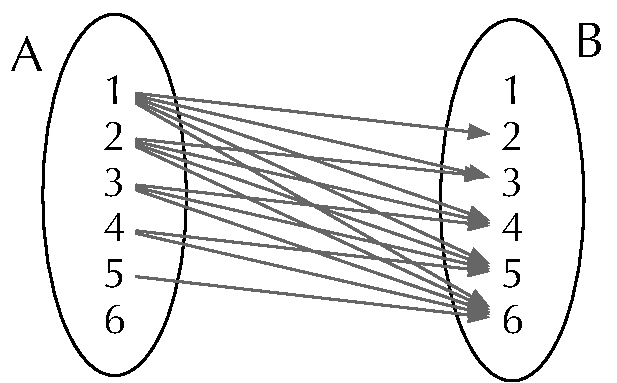
\includegraphics[width=6cm]{pic/RelDigraph.pdf}
\qquad
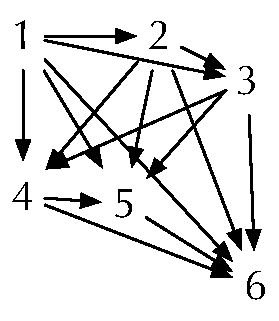
\includegraphics[width=3cm]{pic/RelOneDigraph.pdf}
\end{center}
\caption{The ``strictly smaller'' relation described by digraphs}
\label{figRelDigraph}
\end{figure}

A further variant of this description is the \defini{digraph} (short for
``directed graph''). We draw the sets $A$ and $B$ on two sides and connect
element $a\in A$ to $b\in B$ by an arrow, whenever $(a,b)\in R$.
Figure~\ref{figRelDigraph}, left depicts this for the example.
\smallskip

If, as in this example, we have that $A=B$, we could also draw arrows between elements
of $A=B$.

\medskip

The second way of description is to give a predicate that 
identifies the pairs in relation. In the example, this predicate would be:
$S(a,b)$ if
$a<b$. It then is often convenient to write the predicate as a connecting
symbol, i.e. $3S5$. You have used symbols such as $\le$,
$\subset$, or $\in$ before, formally they all denote relations.
\medskip

\begin{figure}[t]
\begin{center}
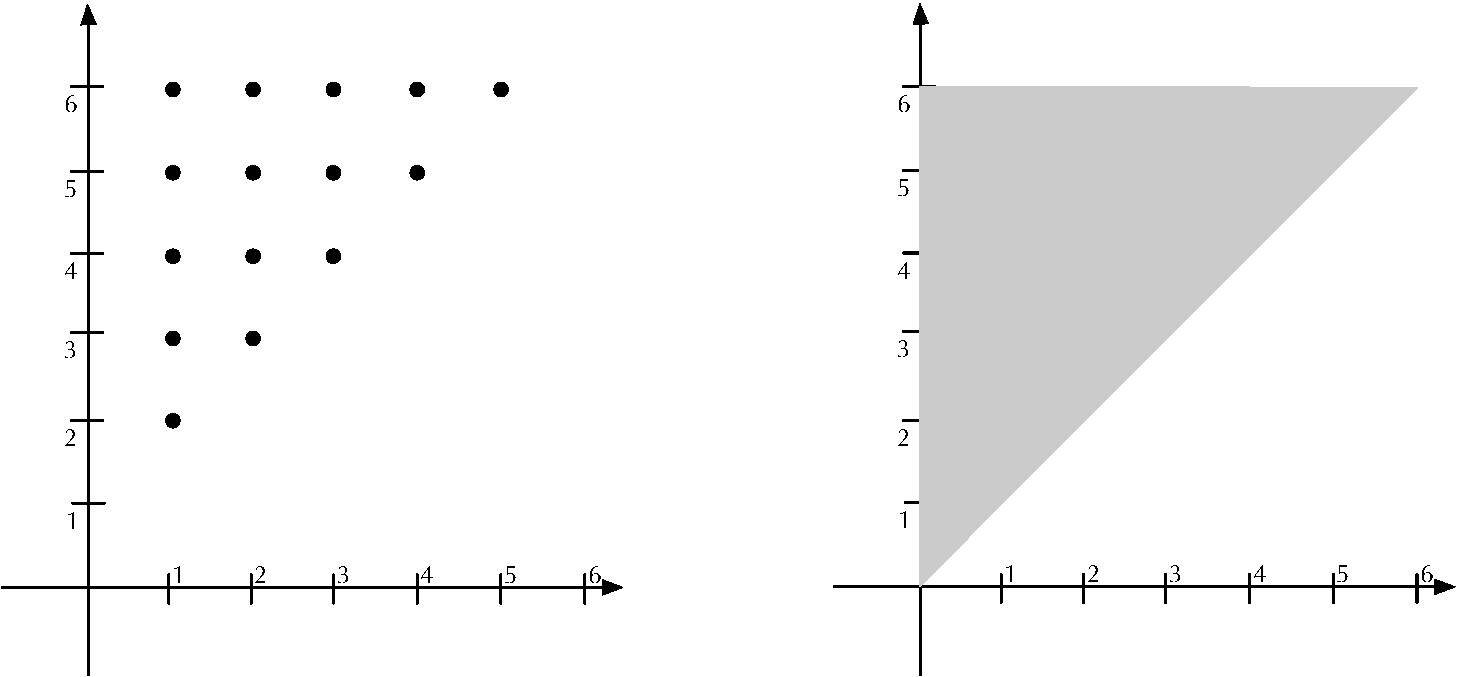
\includegraphics[width=10cm]{pic/StrictlySmallerRel.pdf}
\end{center}
\caption{The strictly smaller relation on integers and on real numbers}
\label{figsmaller}
\end{figure}

The third way of describing relations is one you will have seen before, but
maybe not under this name. Assume that we can arrange the sets $A$ and $B$
along a line. (This is easy if $A$ and $B$ are subsets of the rational or
the real numbers.)
We then can interpret the pairs $(a,b)$ in relation as coordinates of points
in the plane $A\times B$.
We call this the \defini{graph} of the
relation. Figure~\ref{figsmaller}, left, shows the graph of the ``strictly
smaller'' relation on $A=\{1,2,\ldots,6\}$, the right image then shows the
graph of the same relation on the set $B=\{0\le x\le 6\}\subset\R$.

\begin{figure}[t]
\begin{center}
\begin{tabular}{lll}
\begin{minipage}[t]{3.5cm}
a) $x^2+y^2=1$\\
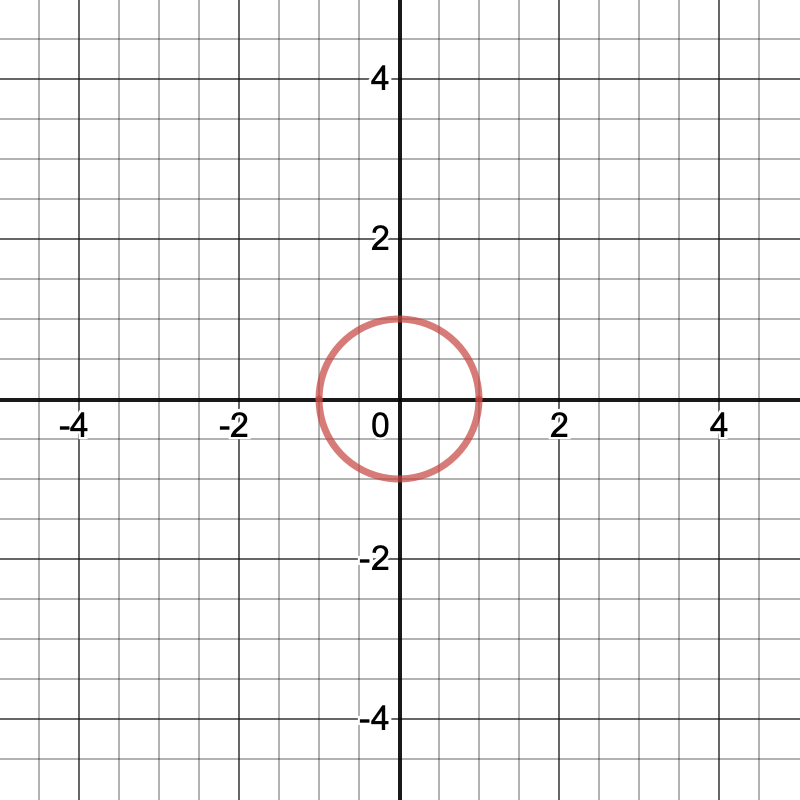
\includegraphics[width=3cm]{pic/relsample1.png}
\end{minipage}&\begin{minipage}[t]{3.5cm}
b) $y=x^2$\\
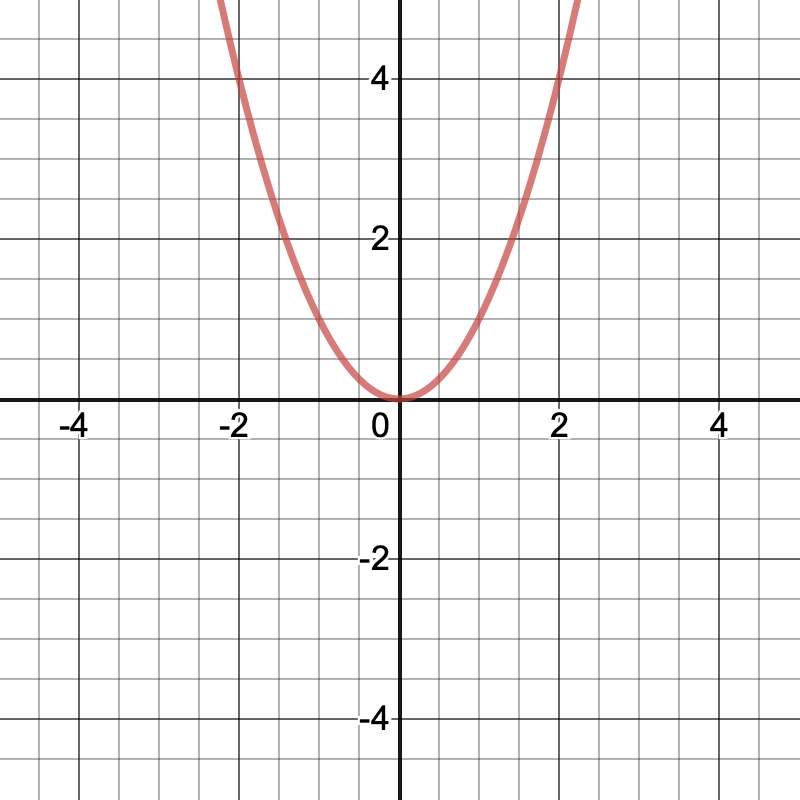
\includegraphics[width=3cm]{pic/relsample2.png}
\end{minipage}&\begin{minipage}[t]{3.5cm}
c) $x=y^2$\\
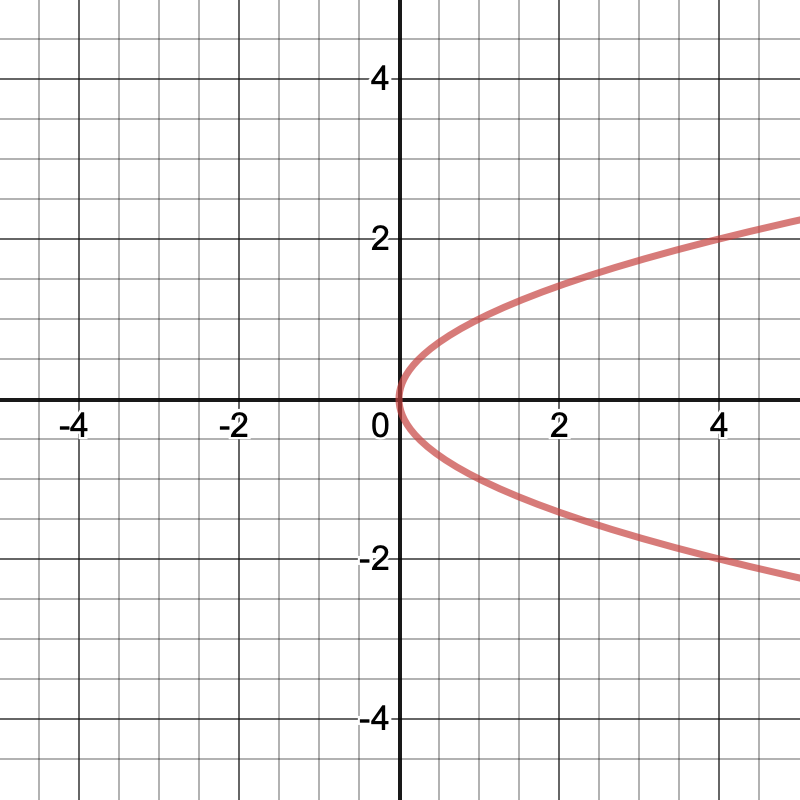
\includegraphics[width=3cm]{pic/relsample3.png}
\end{minipage}\\
\\
\begin{minipage}[t]{3.5cm}
d) $y^2=x^3-3x+1$\\
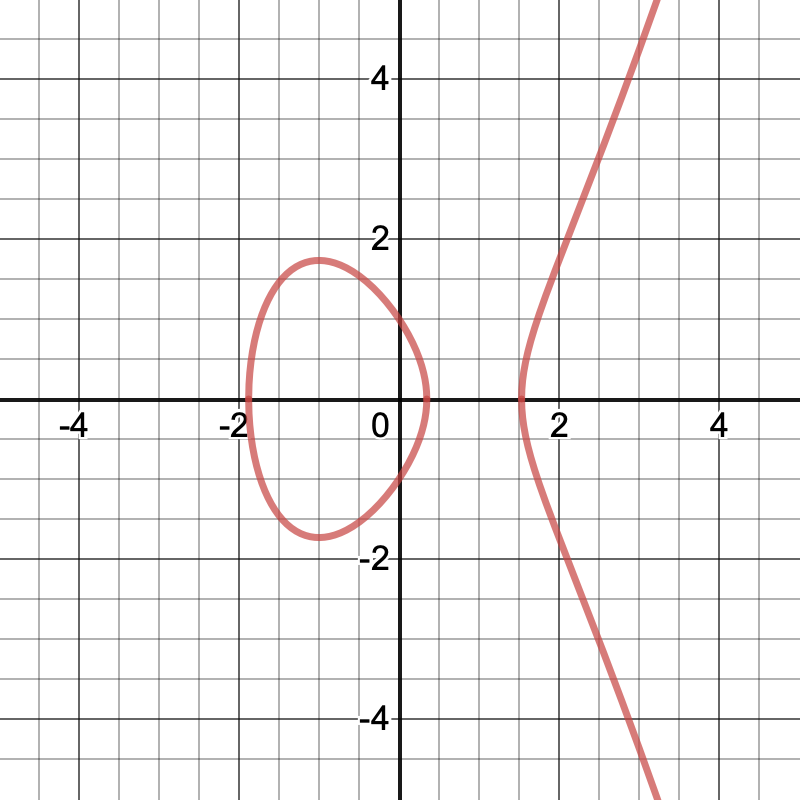
\includegraphics[width=3cm]{pic/relsample4.png}
\end{minipage}&\begin{minipage}[t]{3.5cm}
e) $|x-y|\le 1$\\
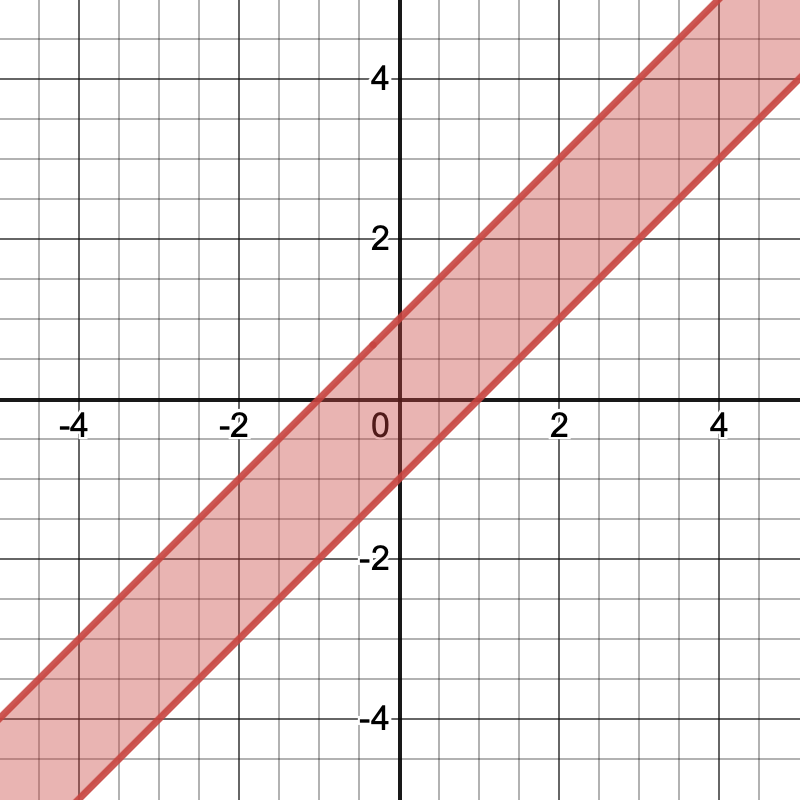
\includegraphics[width=3cm]{pic/relsample5.png}
\end{minipage}&\begin{minipage}[t]{3.5cm}
f) $2\le x,y\le 3$\\
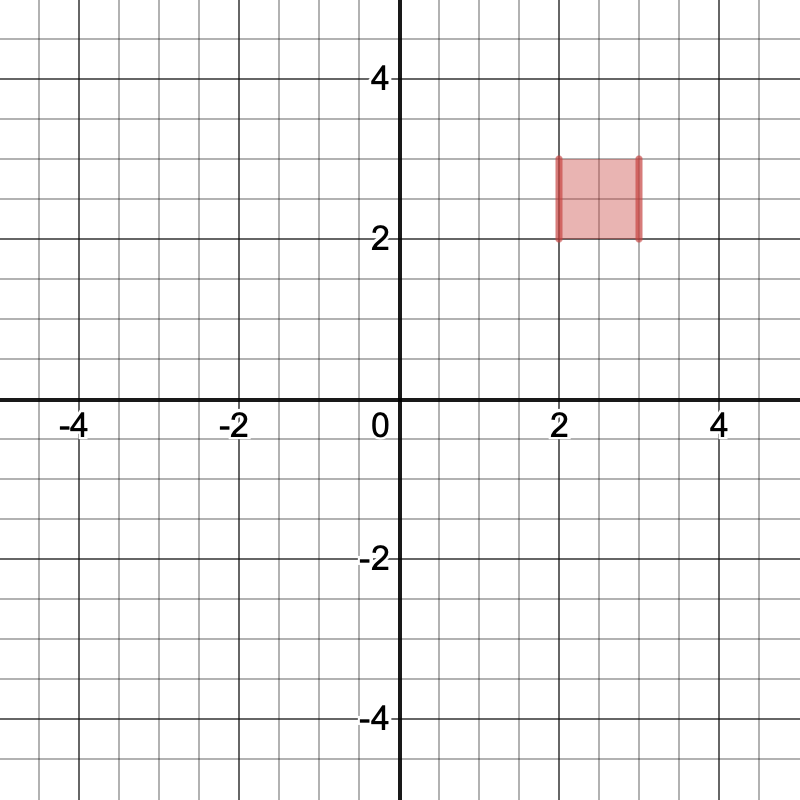
\includegraphics[width=3cm]{pic/relsample6.png}
\end{minipage}\\
\\
\begin{minipage}[t]{3.5cm}
g)$x,y\in\Z$\\
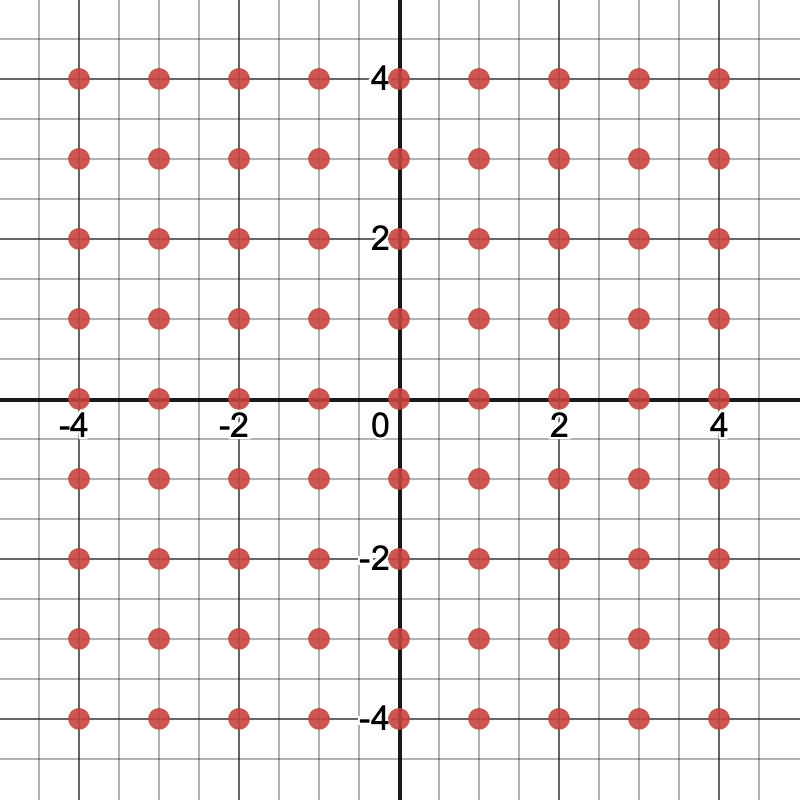
\includegraphics[width=3cm]{pic/relsample7.png}
\end{minipage}&\begin{minipage}[t]{3.5cm}
h) (Too complicated for formula)\\
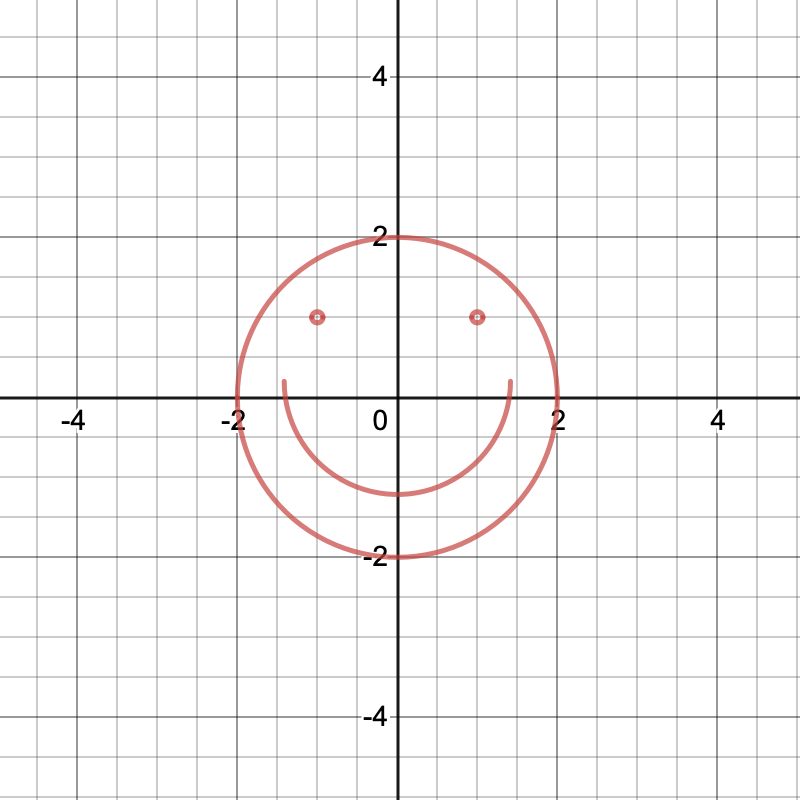
\includegraphics[width=3cm]{pic/relsample8.png}
\end{minipage}&\begin{minipage}[t]{3.5cm}
i) $x+y\in\Z$\\
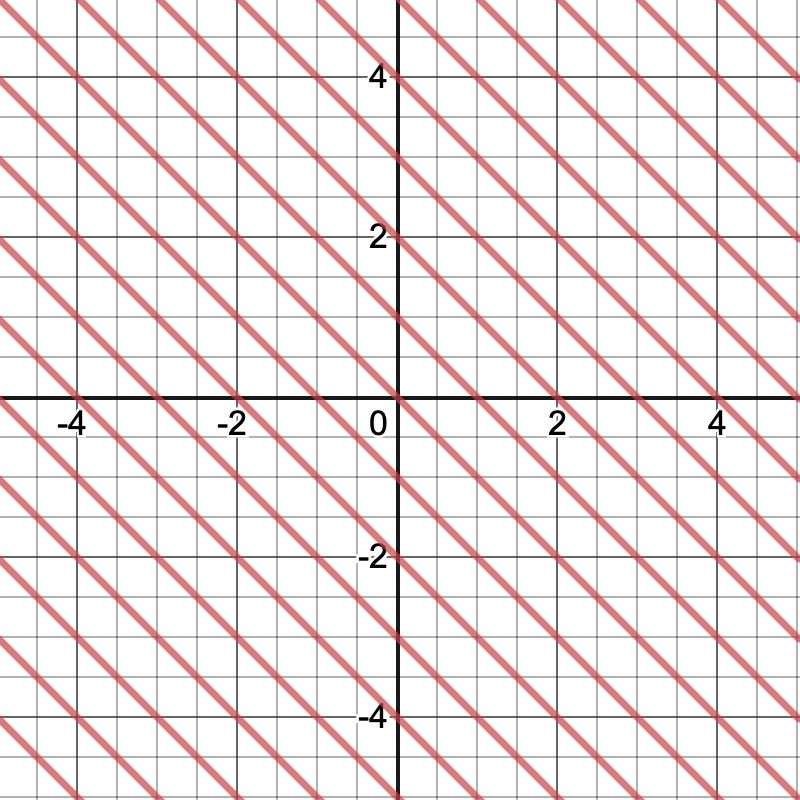
\includegraphics[width=3cm]{pic/relsample9.png}
\end{minipage}\\
\end{tabular}
\end{center}
\caption{Some relations on $\R\times\R$}
\label{figsomeRelations}
\end{figure}

A number of further examples are shown in
\figuref{figsomeRelations}. In all of these examples we have $A=B=\R$ and
indicate the condition for a pair $(x,y)$ to be in the relation.

\subsection{Domain, Range, Source and Target}

To talk about relations, it will be useful to define a number of terms.
\begin{defn}
Let $R\subset A\times B$ a relation. We call $A$ the \defini{source} of $R$
and $B$ the \defini{target} of $R$.

The set
\[
\{a\in A\mid (a,b)\in R\mbox{\ for some $b\in B$}\}\subset A
\]
is called the \defini{domain} of $R$, while
\[
\{b\in B\mid (a,b)\in R\mbox{\ for some $a\in A$}\}\subset B
\]
is called the \defini{range} of $R$.
\end{defn}

In the above example of the strictly smaller relation on $A=B=\{1,\ldots,6\}$,
we have that source and target are both equal to $A=B$. The domain is
$\{1,2,3,4,5\}$ (as $6$ is not smaller than any number), while the range is
$\{2,3,4,5,6\}$.

\section{Complements, Converse and Composition}

Sometimes it can be convenient to build new relations from existing ones --
e.g. the relation of ``parent'' implies also the relations of ``child'' and
of ``grandparent''. Here are some ways to build new relations from old ones.
\medskip

The first observation is that a relation is a set and thus subject to set
operations. If $R\subset A\times B$ is a relation, the complement
\[
R^\mycomplement=\{(a,b)\mid (a,b)\not\in R\}\subset A\times B
\]
is the logical negation with $aR^\mycomplement b$ if and only if
$a\not\sim_R b$. For example,
if we take for $R$ the relation ``parent'', then $R^\mycomplement$ is the
relation ``is not parent''.
\medskip

The next operation is that we swap the pairs in $R$ around (or reverse the
direction of the arrows in the digraph representation). This is called the
\defini{converse} of $R$. Formally we define the converse as
\[
\{(b,a)\in B\times A\mid (a,b)\in R\}.
\]
For example if $R$ is the relation ``is parent of'', then its converse is
the relation ``is child of''.
\medskip

The third operation turns out the most useful, but also maybe most
complicated one. Here we take two relations $R\subset A\times B$ and
$S\subset B\times C$ such that the target of the first relation is the
source of the first. The \defini{composition} of $R$ with $S$ is the
relation 
\begin{eqnarray*}
S\circ R&=&\{(a,c)\in A\times C\mid \exists b\in B: (a,b)\in R\mbox{\ and\
}(b,c)\in S\}\\
&=&\{(a,c)\in A\times C\mid (a,b)\in R\mbox{\ and\ }(b,c)\in S
\mbox{\ for an element $b\in B$}\}
\end{eqnarray*}
Note that we write the composition in {\em reverse order} as $S\circ R$,
with a circle $\circ$ as connection. (Why so? Because it fits with how
functions are used, as we will see later~\pointer{secfunccomposition}\.)

For example, if $R$ is the relation ``is parent of'' and $S$ is the relation
``is spouse of'', then $S\circ R$ is ``parent of spouse'' or
``parent-in-law'' -- $aRb$ and $bSc$ means that $a$ is parent of $b$ and $b$
is spouse of $c$.  On the other hand, $R\circ S$ is ``spouse of parent''
(that is parent or step-parent),
\smallskip

Composition is probably easiest visualized in the digraph model. We are
connecting $a\in A$ to all $c\in C$ that can be reached by following arrows
from $a$ through elements $b\in B$.

For example, with $A=\{1,2,3,4\}$, $B=\{p,q,r,s\}$ and $C=\{w,x,y,z\}$,
Figure~\ref{figcompdig}, left, shows the two relations
$R=\{(1,q),(3,p),(3,s),(4,q)\}$ as well as $S=\{(p,y),(p,z),(q,x),(r,w)\}$. On the
right then is seen the composition $S\circ R=\{(1,x),(3,y),(3,z),(4,x)\}$.
Note that the fact that $3Rs$ or $rSw$ do not contribute to the composition.
\begin{figure}[t]
\begin{center}
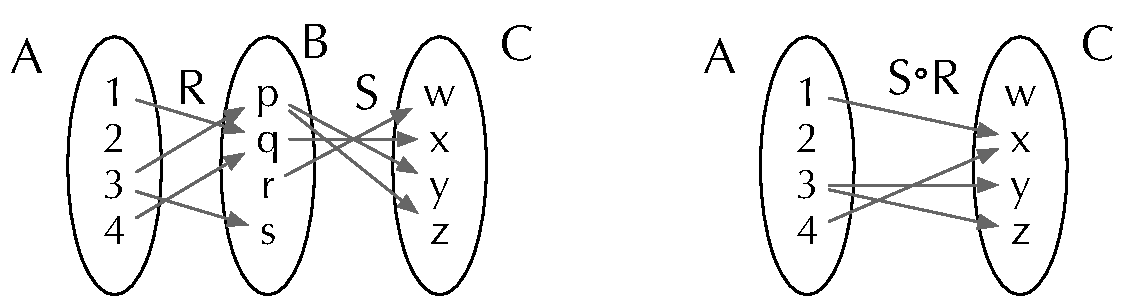
\includegraphics[width=10cm]{pic/CompositionDigraph.pdf}
\end{center}
\caption{Composition of relations}
\label{figcompdig}
\end{figure}

Composition is useful in that it can form genuinely new connections between
objects. 

(In the case of higher order relations (and relational databases),
composition generalizes to an operation {\em join}.)

\section{Properties of Relations}

We shall focus, for a while, on binary relations on a set $A$ (that is
relations amongst elements of one set $A=B$). We first
define a number of
properties that such a relation might have:
\begin{figure}
\begin{center}
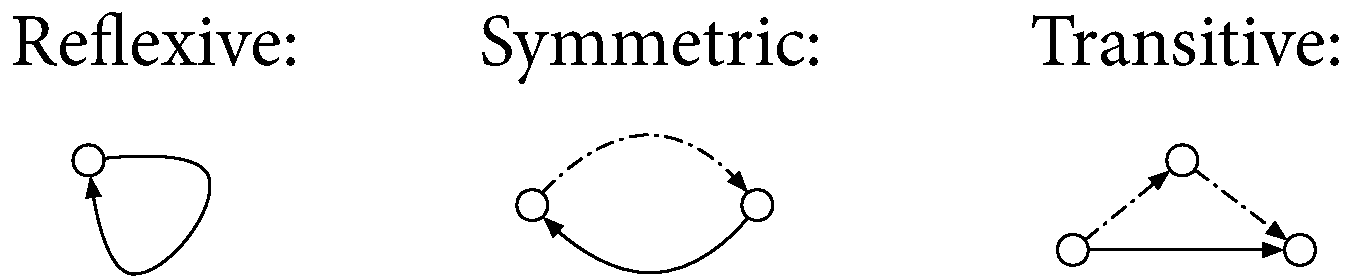
\includegraphics[width=8cm]{pic/RepPropsDigraph}
\end{center}
\caption{Possible Properties of a Relation}
\label{figreppropsdigraph}
\end{figure}
\begin{defn}
Let $\sim$ be a binary relation on a set $A$. Then $\sim$ is called
\begin{description}
\item[\defini{reflexive},] if $a\sim a$ for every $a\in A$.
\item[\defini{symmetric},] if (for $a,b\in A$) $a\sim b$ implies that $b\sim a$.
\item[\defini{antisymmetric},] if (for $a,b\in A$) $a\sim b$ and $b\sim a$ together
imply that $a=b$. (This means that, apart from a trivial case we might have either
$a\sim b$ or $b\sim a$, but not both. Think of the $\le$ relation on numbers.)
\item[\defini{transitive}], if (for $a,b,c\in A$) $a\sim b$ and $b\sim c$ imply that
$a\sim c$.
\end{description}
\end{defn}
In the digraph model (with one set, identifying $A$ and $B$, a relation is
reflexive if there is an arrow from every vertex to itself, it is symmetric,
if for every arrow there is an arrow in the opposite direction, and it is
transitive, if for every pair of arrows following each other, there is a
``composite arrow''. Figure~\ref{figreppropsdigraph} illustrates this (the full
lines are required, if the dashed lines exist).

We give some examples: 
\begin{enumerate}
\item
Let $A$ be the set of rational numbers and $R$ be ordinary equality. (That is 
\[
R=\{(a,b)\in\Q\times\Q\mid a=b\}.)
\]
This relation is reflexive, symmetric and transitive
\item
Let $A$ be the set of all people in a country with two people in relation if they have
the same last name. This relation is reflexive, symmetric and transitive.
\item
Let $A$ be the set of all people living in the United
States\mynote{Constitutional
scholars should take the continental US without Washington DC here} with two people in
relation if they live in the same state. Again this relation is reflexive, symmetric and
transitive.
\item
\label{expointpairs}
Let $A=\R\times\R$ the set of points in the plane, with two points in relation
if they have the same $x$ coordinate or the same $y$ coordinate. (That is, one could
draw a horizontal line or a vertical line through the two points.)
We practice the set notation for relations by writing this down formally, noting that
we have to describe pairs of pairs:
\[
R=\{((x,y),(a,b))\in A\times A\mid x=a \mbox{\ or\ }y=b\}.
\]
This relation is reflexive and symmetric, but not transitive (go first horizontal, then
vertical).
\item
We slightly modify example~\ref{expointpairs} by requiring same $x$ or same $y$
coordinate, but not both the same. Then the relation is only symmetric, but not
reflexive any more.
\item
Let $A$ be a set and $R=A\times A$ (i.e. all elements are in relation). This relation
is reflexive, symmetric and transitive.
\item
Let $A$ be an arbitrary nonempty set and $R=\emptyset$ (that is no elements
are in relation). Then $R$ is symmetric and transitive (both conditions are
true\mynote{This situation of true statements is sometimes called
\defini{vacuously true}} since they are ``if-then'' with a condition that
never can be fulfilled.), but not reflexive.
\item Let $A=\Q$ with the usual ``smaller or equal'' relation $\le$. This relation is
reflexive, antisymmetric and transitive, but not symmetric.
\item Let $A=\Q$ with the ``strictly smaller'' relation to be smaller but not equal. 
This relation is antisymmetric (again vacuously as it is not possible that $a<b$ and
$b<a$ for inequal $a,b$) and transitive, but not reflexive.
\item The relation $x^2+y^3=1$ on $\R$ has none of these properties.
\end{enumerate}

For the graph of a relation defined on (subsets) of $\R$, reflexivity (that is $(x,x)\in
R$) means that the (increasing) diagonal through the origin must be part of the graph.
Symmetry means that the graph is symmetric when reflecting along this diagonal.
(Transitivity is somewhat more complicated and probably less helpful to visualize.)

\section{Equivalence Relations, Equivalence Classes and Partitions}
\label{secequiv}

Restricting our focus even more,
we now consider relations that could be used to represent a concept of
equality. This is an idea
you have used before easily. For example you probably would
claim that $3=\mbox{\Huge 3}$, even though the digits are of different
size\mynote{On the other hand, if your business is in selling house numbers,
you might consider them different, as you will be charging more for the
larger digit.}. But they represent the same magnitude. Some of the examples in the
last section share this characteristic, and we will characterize it with the
properties we just defined:
\begin{defn}
A binary relation $\sim$ on a set $A$ is an \defini{equivalence relation} if
it is reflexive, symmetric and transitive.
\end{defn}
Equivalence relations can be though of as a ``less picky'' version of
\defini{equality} that allow us to forget about differences between objects (say the
color or size  of (physical) numbers). Often one deliberately wants to
consider formally different things as the same. 

This concept of different levels of ``being the same'' occurs naturally in
everyday life. For example, if we say that {\em all persons are equal}, we do not
mean that they are identical (and that there is but one person in the world), but
that they have the same natural rights and privileges.

For a more mathematical example, consider the expressions $1+1$ and $2$, they are formally
different objects (and a typesetter certainly will consider them as not
the same. But if we consider them as expressing magnitudes, we say that
$1+1=2$.
This can be described as an equivalence relation on algebraic expressions.
\medskip

An important characterization of equivalence relations is that they chop a
set into parts, allowing for example for clustering large sets of data into
a smaller number of cases. We shall investigate this next.
\begin{defn}
Let $A$ be a set. A \defini{partition} of $A$ is a set $P$ consisting of nonempty
subsets $S\subset A$ (often called \defini{cells}), such that:
\begin{enumerate}
\item No two different subsets share an element\mynote{This is a somewhat slick
definition. You probably would have written ($S=T$ or $S\cap T=\emptyset$). 
Doings so would
describe the same (logic), but the way we write it down here makes verifying the property
less work to write.}:
\[
\forall S,T\in P: (S\cap T\not=\emptyset\Rightarrow S=T).
\]
\item Every element of $A$ is in a subset: 
\[
\forall a\in A\exists S\in P: a\in S.
\]
\end{enumerate}
\end{defn}
For example, we could take $A=\{1,2,3,4,5\}$ and 
\[
P=\{\{1,3\},\{2,4,5\}\}.
\]
Note that $P$ is not a subset of $A$, but if $S\in P$ then $S\subset A$.

\begin{lemma}
Let $P$ be a partition of $A$. Then every element of $A$ is in exactly one $S\in P$.
\end{lemma}
\begin{proof}
By the second property it needs to be in at least one set, by the first property it
cannot be in more than one.
\end{proof}

If $S\in P$ and $a\in S$, we call $a$ a \defini{representative} of $S$.  It often is
convenient to describe cells by giving such a representative.
Typically representatives are not unique. Indeed, by the prior lemma, any
element of a cell can serve as its representative.
\bigskip

We now want to show that partitions and equivalence relations are closely related.

Given a partition $P$ of $A$, we define a relation on $A$ by
defining $a\sim b$ if and only if $a$ and $b$ are in the {\em same} set of
the partition. In the example above, this would yield the relation
\[
\begin{split}
RP=\{&(1,1),(2,2),(3,3),(4,4),(5,5),\\
&(1,3),(3,1),(2,4),(4,2),(2,5),(5,2),(4,5),(5,4)\}
\end{split}
\]
Such a relation is clearly an equivalence relation: an element is in the
same set as itself. If $a$ and $b$ are in the same set, so are $b$ and $a$,
and if $a$ and $b$, as well as $b$ and $c$ are in the same set, this set
contains $a$ and $c$.

The same holds in reverse. For this, assume we are given an equivalence
relation $\sim$ on a set $A$. For every $a\in A$ we 
define its \defini{equivalence class} as the set of all elements in relation
to $a$:
\[
[a]=\{b\in A\mid b\sim a\}.
\]
Clearly $a\in[a]$ is in its own equivalence class, and equivalence classes
thus are not empty, and every element of $A$ lies in an equivalence class.
We also note that if $a\sim b$, then $[a]=[b]$, since any $c\in[a]$
satisfies $c\sim a$ and thus $c\sim b$ by transitivity (and vice versa for
$c\in[b]$). Thus, if two equivalence classes have non-empty intersection,
they are equal: let $c\in [a]\cap [b]$, then $c\sim a$, $c\sim b$ (and
thus $b\sim c$
because of symmetry) and by transitivity $b\sim a$ and thus $[a]=[b]$.

This means that the set of equivalence classes forms a partition of the set
$A$. If $a$ is the representative of a class $S$, then $S=\{b\in A\mid b\sim a\}$.

In the above example, the relation  $RP$
creates the equivalence classes
\[
\{1,3\}\mbox{\ and\ }\{1,4,5\},
\] and thus the partition $P$.

For another, prototypical, example, suppose we define a relation $\sim$ on the set $\Z$ of
integers by defining $a\sim b$ if $2$ divides $a-b$. Then we get two
(infinitely large)
equivalence classes, namely the even and the odd numbers. If we change the
equivalence to $a-b$ being divisible by $3$, we get three
(infinite) equivalence classes:
\[
\{0,3,-3,6,-6,\ldots\},\quad
\{1,4,-2,7,-5,\ldots\},\quad
\{2,5,-1,8,-4,\ldots\}.
\]
Equivalence classes will be important tools for us to construct new classes
of objects, in particular arithmetic objects.
\medskip

\begin{figure}[t]
\begin{center}
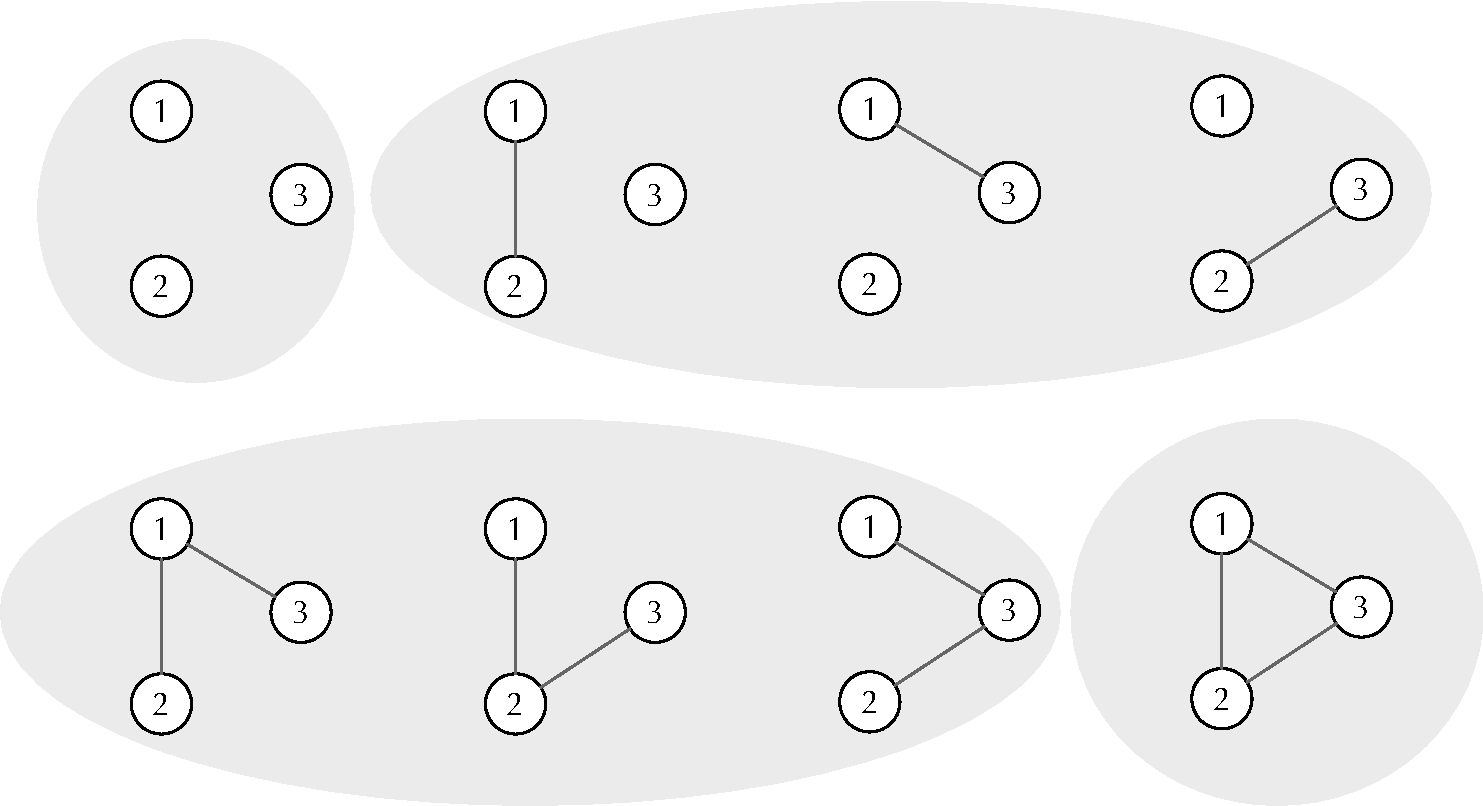
\includegraphics[width=10cm]{pic/GraphIsoClasses.pdf}
\end{center}
\caption{The possible graphs on 3 vertices}
\label{3vertexgraphs}
\end{figure}

For a more elaborate example of equivalence classes, and why we care about
them, consider graphs. A graph consists of \defini{vertices} (basically
points), together with \defini{edges} that each connect two vertices.

To represent a graph, we need to represent the vertices -- say for a graph
on $n$ vertices with the numbers $1,2,\ldots,n$. An edge then is a set of
two vertices. For example (\figuref{3vertexgraphs}) consider graphs on $n=3$
vertices. There are 3 potential edges and each edge can be selected or not,
so we get $2^3=8$ possibilities for \defini{labelled graphs}, that is graphs
where the labeling of the vertices matters.

But often we do not care about this labeling but only  about the possible
connection patterns. We thus can define an equivalence relation
(called~\defini{graph isomorphism}, this is an important, hard, algorithmic
problem) 
as two graphs being equivalent if they become the same after a
relabeling of the vertices. For example, the graph with the edge set
$\{\{1,2\}\}$ can be transformed into the graph with edge set $\{\{2,3\}\}$ by
relabeling\mynote{This
is not unique. Another option would be $\begin{array}{c}1\to
3\\2\to2\\3\to1\end{array}$.} 
the vertices $\begin{array}{c}1\to 2\\2\to3\\3\to1\end{array}$.

We thus get (for the example of three vertices) $4$ equivalence classes
(as indicated by shaded areas in the figure). These equivalence classes are
what one considers typically as (unlabeled) graphs and the objects one would
like to classify. On the other hand, when storing a graph on the computer,
one needs to identify vertices in some way, which (implicitly) gives them
labels. What is stored is thus a labeled graph as representative of its
conjugacy class.

\section{The Integers and the Rationals}

In the remainder of this chapter we study a number of examples in which
equivalence relations or equivalence classes are used to construct
interesting objects.
\smallskip

The first example is to construct (all, including the negative) integers
from the positive numbers (that correspond to counting objects). This
requires more than adding a possible minus-sign, since we need that $-0=0$.
Instead we form equivalence classes on pairs:

Let $\N_0=\{0,1,2,3,\ldots\}$ be the set of nonnegative integers. We form
the set of pairs
\[
S=\N_0\times\N_0=\{(a,b)\mid a,b\in\N_0\}.
\]
Our goal is to have the integer $z$ to be represented by the set
$\{(a,b)\in S\mid b-a=z\}$. To define this set as an equivalence class, we
want to define a relation on $S$ that $(a,b)$ is related to
$(c,d)$, if $b-a=d-c$. Since this might involve negative numbers (which we
are just constructing), we use instead: $b+c=a+d$:
\[
(a,b)\sim(c,d)\Leftrightarrow b+c=a+d.
\]
This relation is clearly reflexive (as $b+a=a+b$) and symmetric (if
$b+c=a+d$ then $d+a=c+b$). For transitivity, observe that if
$(a,b)\sim(c,d)$ then $b+c=a+d$, and if $(c,d)\sim(e,f)$ then $d+e=c+f$. We
add $f$ to the first equation and $b$ to the second and obtain
\[
b+c+f=a+d+f\ \mbox{and}\ b+d+e=b+c+f,
\]
and thus $a+d+f=b+d+e$. But that implies that $a+f=b+e$, and thus
$(a,b)\sim(e,f)$.

We then define arithmetic on the equivalence classes using representatives:
\[
[(a,b)]+[(c,d)]=[(a+c,b+d)]
\]
Formally, we need also to show that this definition is independent of the
choice of representative, that is if $(a,b)\sim(e,f)$ then
$[(a,b)]+[(c,d)]=[(e,b)]+[(c,d)]$, but we skip this somewhat technical step
here.
\bigskip

\subsection{Constructing the rational numbers}

The rational numbers, $\Q$, similarly can be constructed as pairs of
integers,
representing fractions. We start with the set
\[
S=\Z\times (\Z\setminus\{0\})=\{(n,d)\mid n,d\in\Z,d\not=0\}.
\]
Now observe that $n/d=m/e$ if and only if $ne=md$. We thus define a relation
\[
(a,b)\sim(c,d)\Leftrightarrow ad=bc.
\]
As above, one shows easily that this is an equivalence relation. The details
of this are left as an exercise for the reader. One then
defines arithmetic operations on the equivalence classes that mimic the
arithmetic rules for fractions.

\section{Remainders and Modulo}

For the last example, we choose a positive integer $m>1$ and (similar to an
example above) define a relation on $\Z$ by
\[
a\sim b\Leftrightarrow m\mid (b-a)
\]
using the vertical line $\mid$ as a shorthand for ``divides''.  Dividing
means that there exists a $q$ (depending on $b-a$) such that $mq=b-a$.
For example, if we had chosen $m=7$ we would have $3\sim 10$, but $3\not\sim
5$.

Again, we show first that this defines an equivalence relation: Reflexivity
holds as $m\cdot 0=0=a-a$. Symmetry follows from the fact that if $mq=b-a$
then $m(-q)=a-b$. And transitivity from the fact that if $a\sim b$ there
exists $q$ such that $mq=b-a$ and if $b\sim c$ there exists $r$ such that
$mr=c-b$. But then
\[
c-a=c-b+b-a=mr+mq=m(r+q)
\]
and thus $m\mid (c-a)$, i.e. $a\sim c$.
\medskip

We thus can form equivalence classes.
To understand what these classes are, we make a number of observations:

\begin{description}
\itemsep0mm
\item[If $a\in\Z$, we have that the class
containing $a$ is]
\[
[a]=\{a,a+m,a-m,a+2m,a-2m,a+3m,\ldots\}=\{a+k\cdot m\mid k\in\Z\},
\]
since the elements equivalent to $a$ are exactly those that differ from $a$
by a multiple of $m$.
\item[In every class $C$ there is a non-negative integer] For if $x\in C$ we
also have that $x+m\in C$.
\item[In every class $C$ there is an element $r\in C$ with $0\le r\lneqq m$]
Take $r\ge 0$ to be the smallest nonnegative element of $C$. Then $r<m$, as
otherwise $r-m\in C$.
\item[This element $r$ is unique,] that is in the class $C$ there cannot be
two different elements $r_1,r_2\in C$ with $0\le r_1,r_2\lneqq m$. Since if
this was, we would have
(without loss of generality\mynote{This is an example of a useful tool in proofs.
We could have $r_1<r_2$ or $r_2>r_1$ and would need to consider both cases.
But there is freedom in labeling the two numbers and we use this freedom 
to dictate that $r_1$ shall be the smaller of the two numbers.
Such a choice does not conflict with any other requirement, and thus is
permissible. This means that such a choice does not restrict the argument to
a special case, but still is applicable to all situations.}
$r_1<r_2$, but then $0<r_2-r_1$
and $m\mid r_2-r_1\lneqq m$, which is impossible.
\item[There are $m$ equivalence classes, namely \hbox{$[r]$}
for $0\le r\lneqq m$.]
This is since each number $0\le r\lneqq m$ must be in an equivalence class,
but no two of them are in the same class. And each class must contain such
an $r$.
\end{description}
Part of these observations are summarized in the following theorem:
\begin{thm}[Division with remainder]
For any integer $m>1$ and any integer $a$, there exist unique $q,r\in\Z$
such that $a=qm+r$ with $0\le r\lneqq m$.
\end{thm}

For example, if we choose $m=3$ there will be $3$ equivalence classes,
namely $[0]=[3]$, $[1]$, and $[2]$.

If the number $m$ is chosen and fixed, sometimes the convention is used to
denote this remainder $r$ by $\overline a$.

\subsection{Modular Arithmetic}

We now define arithmetic on the equivalence classes by the following rules:
\begin{eqnarray*}
\hbox{$[a]+[b]$}&:=&[a+b]\\
\hbox{$[a]\cdot[b]$}&:=&[a\cdot b]\\
\end{eqnarray*}
To ensure there is no ambiguity in which representative we chose, we show that the
result is the same, even if we chose different representatives. Recall, that the
elements of $[a]$ are of the form $a+k\cdot m$ for $k\in\Z$. We thus need to show that
the results of addition and of multiplication yield the same results, even if we replace
$a$ by $a+k\cdot m$ and $b$ by $b+l\cdot m$:
\begin{eqnarray*}
\hbox{$[a+km]+[b+lm]$}&=&[(a+km+b+lm)]=[a+b+m(l+k)]=[a+b]\\
\hbox{$[a+km][b+lm]$}&=&[(a+km)(b+lm)]=[ab+m(al+bk+klm)]=[ab]
\end{eqnarray*}
These results imply that the standard arithmetic rules
we know for integers also hold for these operations on equivalence classes.

We have thus defined a new kind of arithmetic, involving addition, subtraction (from
addition of the negative) and multiplication, on the $m$ equivalence classes
$[0],[1],\ldots,[m]$. It is called \defini{modular arithmetic} (or \defini{modulo}
arithmetic). One often writes
$i\bmod m$ instead of $[i]$.

Using the $\overline\cdot$ notation for remainders, the same result can be
interpreted as
$\overline{a+b}=\overline{\overline{a}+\overline{b}}$ and
$\overline{a\cdot b}=\overline{\overline{a}\cdot \overline{b}}$.
\medskip

Modular arithmetic is particularly well suited for computers, because the set
of objects is finite. Binary arithmetic on bits is just arithmetic modulo
$2$. And standard arithmetic on a 64-bit processor is simply arithmetic
modulo $2^{64}$.  Modular arithmetic also has important applications in data
transmission and information security. You will encounter it again in more
advanced classes.

\subsection{Examples of Modular Arithmetic}

One way of describing modular arithmetic is by giving tables for addition and
multiplication. We do this here, for example, for $m=7$:
\begin{center}
\begin{tabular}{cc}
$\begin{array}{c|ccccccc}
+&\overline{0}&\overline{1}&\overline{2}&\overline{3}&\overline{4}&\overline{5}&\overline{6}\\
\hline
\overline{0}&\overline{0}&\overline{1}&\overline{2}&\overline{3}&\overline{4}&\overline{5}&\overline{6}\\
\overline{1}&\overline{1}&\overline{2}&\overline{3}&\overline{4}&\overline{5}&\overline{6}&\overline{0}\\
\overline{2}&\overline{2}&\overline{3}&\overline{4}&\overline{5}&\overline{6}&\overline{0}&\overline{1}\\
\overline{3}&\overline{3}&\overline{4}&\overline{5}&\overline{6}&\overline{0}&\overline{1}&\overline{2}\\
\overline{4}&\overline{4}&\overline{5}&\overline{6}&\overline{0}&\overline{1}&\overline{2}&\overline{3}\\
\overline{5}&\overline{5}&\overline{6}&\overline{0}&\overline{1}&\overline{2}&\overline{3}&\overline{4}\\
\overline{6}&\overline{6}&\overline{0}&\overline{1}&\overline{2}&\overline{3}&\overline{4}&\overline{5}
\end{array}$
&
$\begin{array}{c|ccccccc}
\cdot&\overline{0}&\overline{1}&\overline{2}&\overline{3}&\overline{4}&\overline{5}&\overline{6}\\
\hline
\overline{0}&\overline{0}&\overline{0}&\overline{0}&\overline{0}&\overline{0}&\overline{0}&\overline{0}\\
\overline{1}&\overline{0}&\overline{1}&\overline{2}&\overline{3}&\overline{4}&\overline{5}&\overline{6}\\
\overline{2}&\overline{0}&\overline{2}&\overline{4}&\overline{6}&\overline{1}&\overline{3}&\overline{5}\\
\overline{3}&\overline{0}&\overline{3}&\overline{6}&\overline{2}&\overline{5}&\overline{1}&\overline{4}\\
\overline{4}&\overline{0}&\overline{4}&\overline{1}&\overline{5}&\overline{2}&\overline{6}&\overline{3}\\
\overline{5}&\overline{0}&\overline{5}&\overline{3}&\overline{1}&\overline{6}&\overline{4}&\overline{2}\\
\overline{6}&\overline{0}&\overline{6}&\overline{5}&\overline{4}&\overline{3}&\overline{2}&\overline{1}
\end{array}$
\end{tabular}
\end{center}

These tables contain many interesting patterns. In the addition table, every row and
every column contain every entry exactly once. The multiplication table (this is because
$m$ is prime, but we shall not prove this here) restricted to $\overline{1}$ to $\overline{6}$ has the same property.
Having $\overline{1}$ in every row and every column means that we can invert every
nonzero number, for example $\overline{1}/\overline{3}=\overline{5}$. This means that
one can solve equations in modular arithmetic as one would do normally. We illustrate
this in the following examples:
\medskip
Consider the equation
\[
4x+3=6\pmod{7}.
\]
We subtract $3$, getting $4x=3\pmod{7}$. We then note from the multiplication table that
$\overline{4}\cdot\overline{2}=\overline{1}$. Multiplying by $2$ thus gives
$x=6\pmod{7}$ as solution.

We can handle systems of equations similarly:
\begin{eqnarray*}
\begin{array}{rcl}
\overline{3}x+\overline{5}y&=&\overline{2}\\
x+\overline{2}y&=&\overline{3}\\
\end{array}
&\Rightarrow&
\begin{array}{rcl}
(\overline{5}-\overline{3}\cdot\overline{2})y=\overline{6}y&=&\overline{2}-\overline{3}\cdot\overline{3}=\overline{0}\\
x+\overline{2}y&=&\overline{3}\\
\end{array}\\
\Rightarrow
\begin{array}{rcl}
y&=&(\overline{1}/\overline{6})\cdot\overline{0}=\overline{0}\\
x+\overline{2}y&=&\overline{3}\\
\end{array}
&\Rightarrow&
\begin{array}{rcl}
y&=&\overline{0}\\
x&=&\overline{3}\\
\end{array}
\end{eqnarray*}


